
%%%%%%%%%%%%%%%%%%%%%%%%%%%%%%%%%%%%%%%%%%%
%%%%%%%Tuo1
To figure out whether we can use previous PM2.5 value to predict future PM2.5 value, we decide to conduct time series analysis. We focus our attention on the PM2.5 site which located at latitude 33.79236 and longitude -118.175 ( It is really close to Long Beach). We collect monthly average PM2.5 concentration value from Jan 2004 to Dec 2014 and plot the time series in the figure below.

\begin{figure}[ht!]
\centering
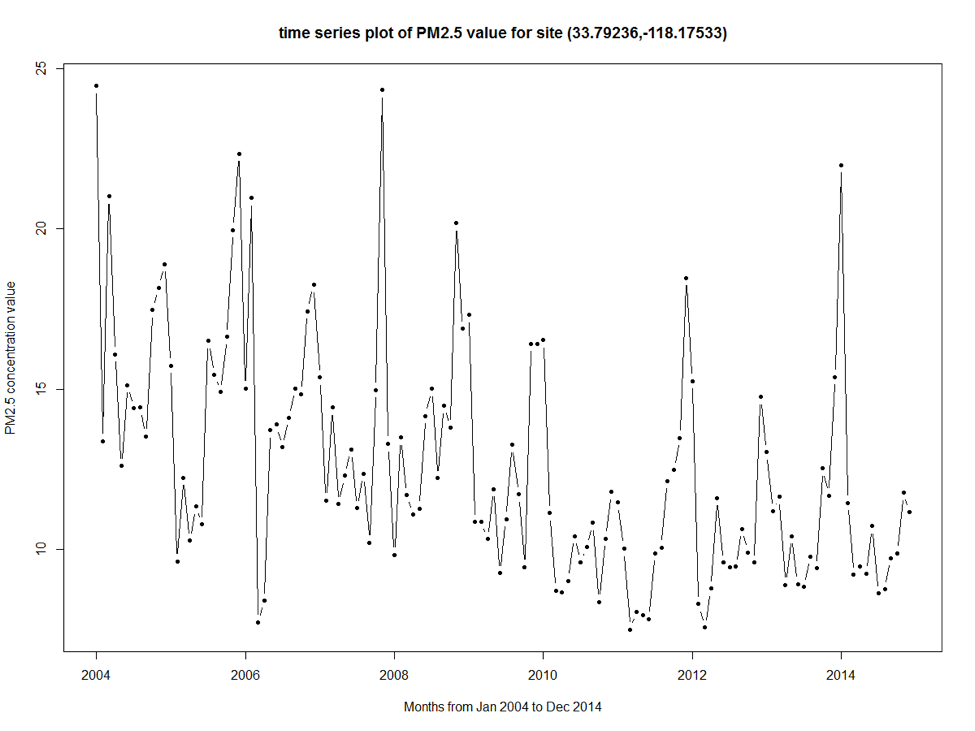
\includegraphics[width = 90mm]{ts1.png}
%\caption{}
%\label{graph4}
\end{figure}

There is a slightly downward trend over time about this time series and there seems to exist seasonality. We decide to use two different methods to fit the time series model. One is Holt-Winters Exponential Smoothing. Exponential smoothing is a very popular scheme to produce a smoothed time series and it assigns exponentially decreasing weights as the observations get older. Holt-Winters Exponential Smoothing can be used to make short-term forecasts on a time series that can be described using an additive model with increasing or decreasing trend and seasonality. The second one is ARIMA model. ARIMA is the short for autoregressive integrated moving average. This model can be fitted to time series data either to better understand the data or to predict future points in the series. For the ARIMA method, we firstly adjust the time series by subtracting the estimated seasonal component and then apply the model to the adjusted series.

%%%%%%end_Tuo1
%%%%%%%%%%%%%%%%%%%%%%%%


%%%%%%%%%%%%%%%%%%%%%%Tuo 2
\subsubsection{Holt-Winters Exponential Smoothing}
We firstly draw fitted value plot based on Holt-Winters Exponential Smoothing. In the plot below, black line represents the variation of real PM value during 2004-2014 and red line represents the variation of fitted PM value during the period. We can see that although the two lines have similar trend, the fitted value is not accurate enough at many points.

\begin{figure}[ht!]
\centering
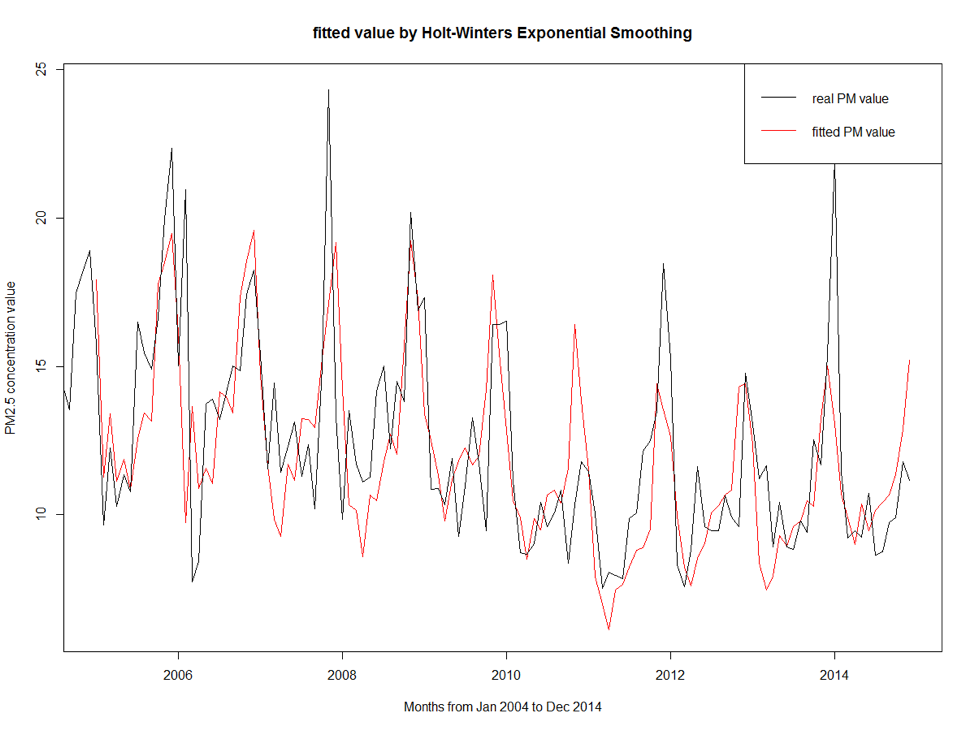
\includegraphics[width = 90mm]{ts2.png}
%\caption{}
%\label{graph4}
\end{figure}

Then we predict the PM2.5 concentration value for the whole year 2015. In the plot below, the blue line represents the predicted value for 2015. The shadow of deep color represents the 80\% prediction interval for the predicted value and the shadow of light color represents the 95\% prediction interval for the predicted value.

\begin{figure}[ht!]
\centering
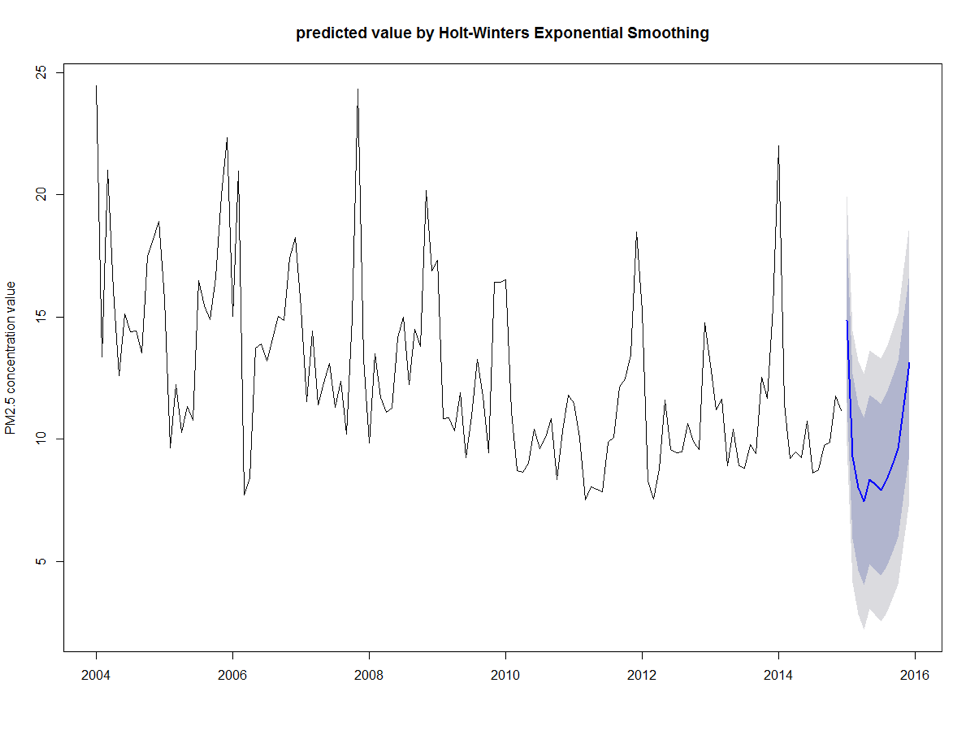
\includegraphics[width = 90mm]{ts3.png}
%\caption{}
%\label{graph4}
\end{figure}

Now let?u exmaine the effect of our prediction. We decide to use mean square error as our criterion. Lower mean square error indicates we have a better prediction. By comparing the predicted results and the real PM value for the year 2015, we find the mean square error between them is around 5.5. Becaues the mean of PM2.5 value during 2004-2014 is about 12.6, the mean square error is kind of large and this model is not very accurate.

\subsubsection{ARIMA model}
Becaues there seems to exist seasonality in the PM2.5 value time series, we want to decompose the time series and apply ARIMA model to the adjusted time series. We first decompose the PM2.5 concentration value time series and plot it. In the plot below, the four subplots respectively represent observed value, overall trend component, seasonal component and random part. From the seasonal component, we can see that there does exist differences of PM2.5 value among different months. By subtracting the seasonal component from the original time series, we get adjusted PM2.5 concentration value time series.

\begin{figure}[ht!]
\centering
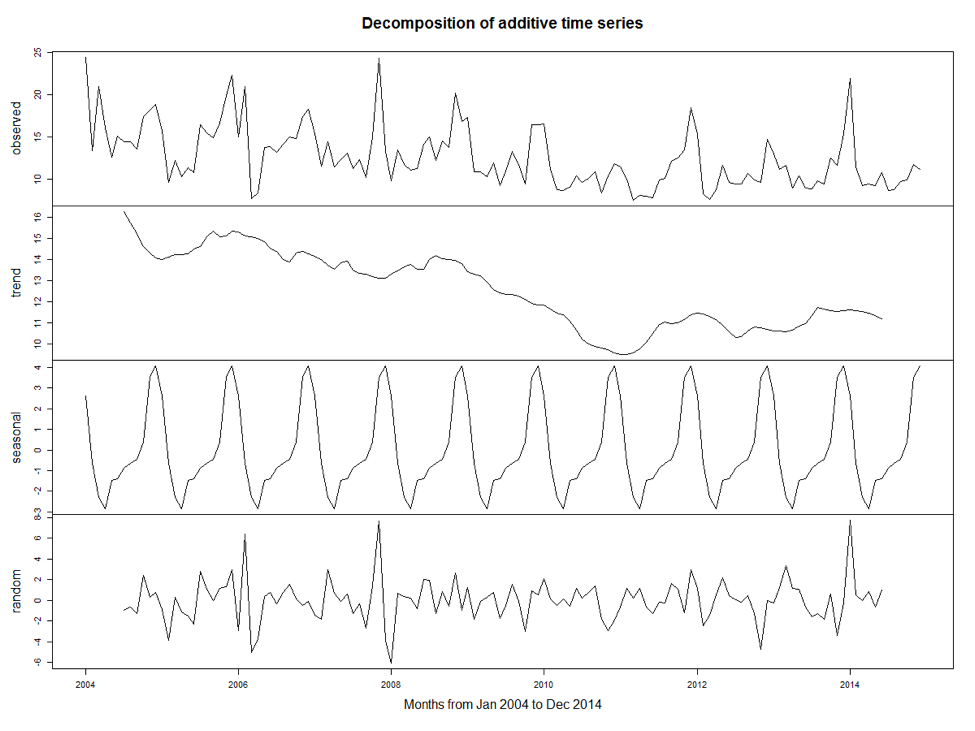
\includegraphics[width = 90mm]{ts4.png}
%\caption{}
%\label{graph4}
\end{figure}

Then we draw fitted adjusted PM value based on ARIMA model, (google). The black line represents the variation of real adjusted PM value during 2004-2014  and red line represents the variation of fitted adjusted PM value during the period. From this plot we can see that the fitted line is really rough.

\begin{figure}[ht!]
\centering
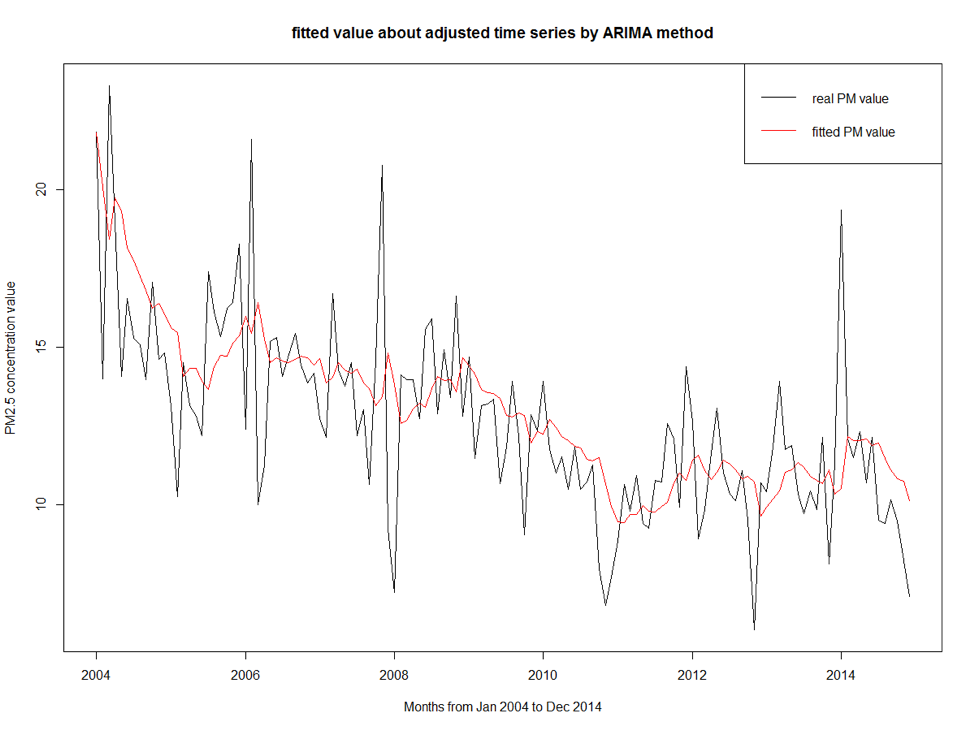
\includegraphics[width = 90mm]{ts5.png}
%\caption{}
%\label{graph4}
\end{figure}

Next, we predict the adjusted PM2.5 concentration value for the whole year 2015. Similar as before, , the blue line represents the predicted value for 2015. The shadow of deep color represents the 80\% prediction interval for the predicted value and the shadow of light color represents the 95\% prediction interval for the predicted value.

\begin{figure}[ht!]
\centering
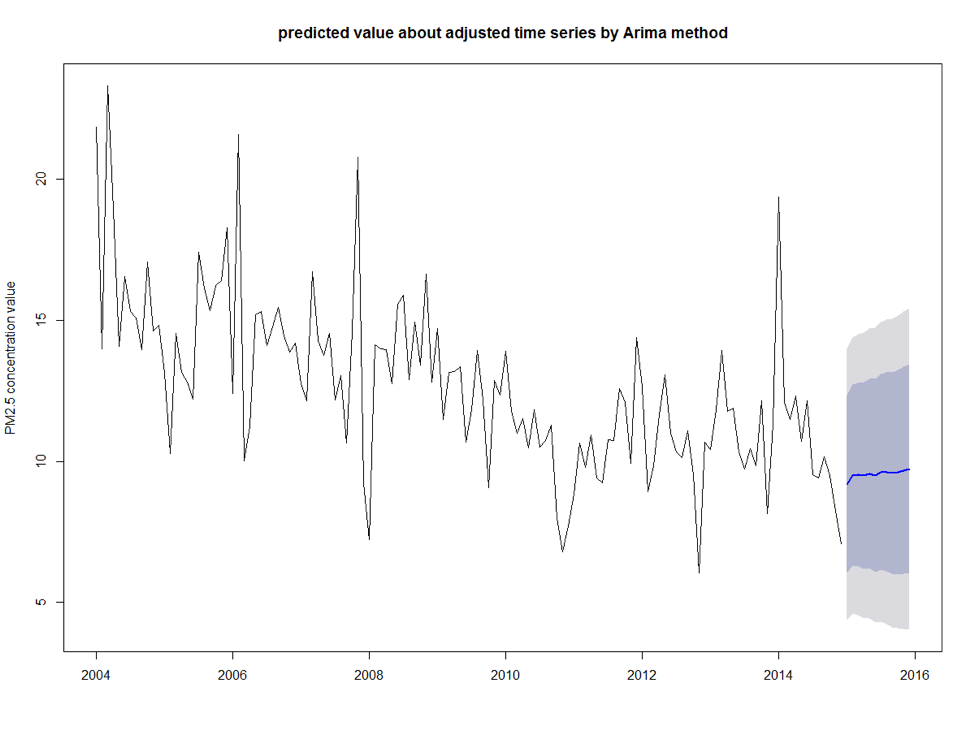
\includegraphics[width = 90mm]{ts6.png}
%\caption{}
%\label{graph4}
\end{figure}

Finally, we adding seasonal component to our predicted result and then compare it with the real PM value during 2004-2014. We find the mean square error is around 9.7. So the performance of ARIMA model is even not as good as Holt-Winters Exponential Smoothing.

In sum, the effect of prediction by time series is not very good. But it does give us some inspiration. For example, the PM 2.5 value will be different in different seasons. For next step
%%%%%%%%%%%%%%%%% End Tuo2


%%%%%%%%%%%Put any citation 

%%%google www.google.com














